\chapter{Catálisis homogénea en la industria}\label{ch:b3:homogeneous-catalysis}

La mayor parte del ácido acético del mundo, materia prima del acetato de vinilo, del
acetato de celulosa y del ácido tereftálico purificado de las botellas de plástico, se
fabrica a partir de metanol y monóxido de carbono en unas pocas plantas muy grandes. En cada una, un
complejo de rodio o de iridio disuelto a baja concentración en el líquido de
reacción efectúa miles de ciclos por hora, durante años. El mismo tipo de
química hidrogena, adiciona CO e hidrógeno a los alquenos, intercambia los extremos de los
dobles enlaces, une anillos aromáticos y fabrica polietileno y polipropileno por
millones de toneladas. Este capítulo lee los ciclos catalíticos de los principales
procesos industriales con las herramientas del \cref{ch:b3:organometallic-bonding}:
recuentos de electrones, estados de oxidación, etapas determinantes de la velocidad y la simetría del
catalizador que fija la estructura de un polímero.

\begin{recall}
El volumen del segundo año introdujo las etapas elementales de las reacciones organometálicas
(adición oxidante, eliminación reductora, inserción migratoria, eliminación de hidruro
en $\beta$, transmetalación), los ciclos catalíticos, los precatalizadores, el número de recambio
y la frecuencia de recambio, y leyó los ciclos de la hidrogenación, la \omterm{def:b3:homogeneous-catalysis:hydroformylation}{hidroformilación} y
el acoplamiento cruzado; definió también la tacticidad y la polimerización en cadena,
la conversión y la selectividad. El \cref{ch:b3:organometallic-bonding} contó
los electrones y describió los ligandos carbonilo y \omterm{def:b3:organometallic-bonding:carbene}{carbeno};
el \cref{ch:b3:complex-kinetics} dio la cinética de saturación, y
el \cref{ch:b3:point-groups}, los \omterm{def:b3:point-groups:operation}{elementos de simetría} de las moléculas.
\end{recall}

\begin{omfigure}
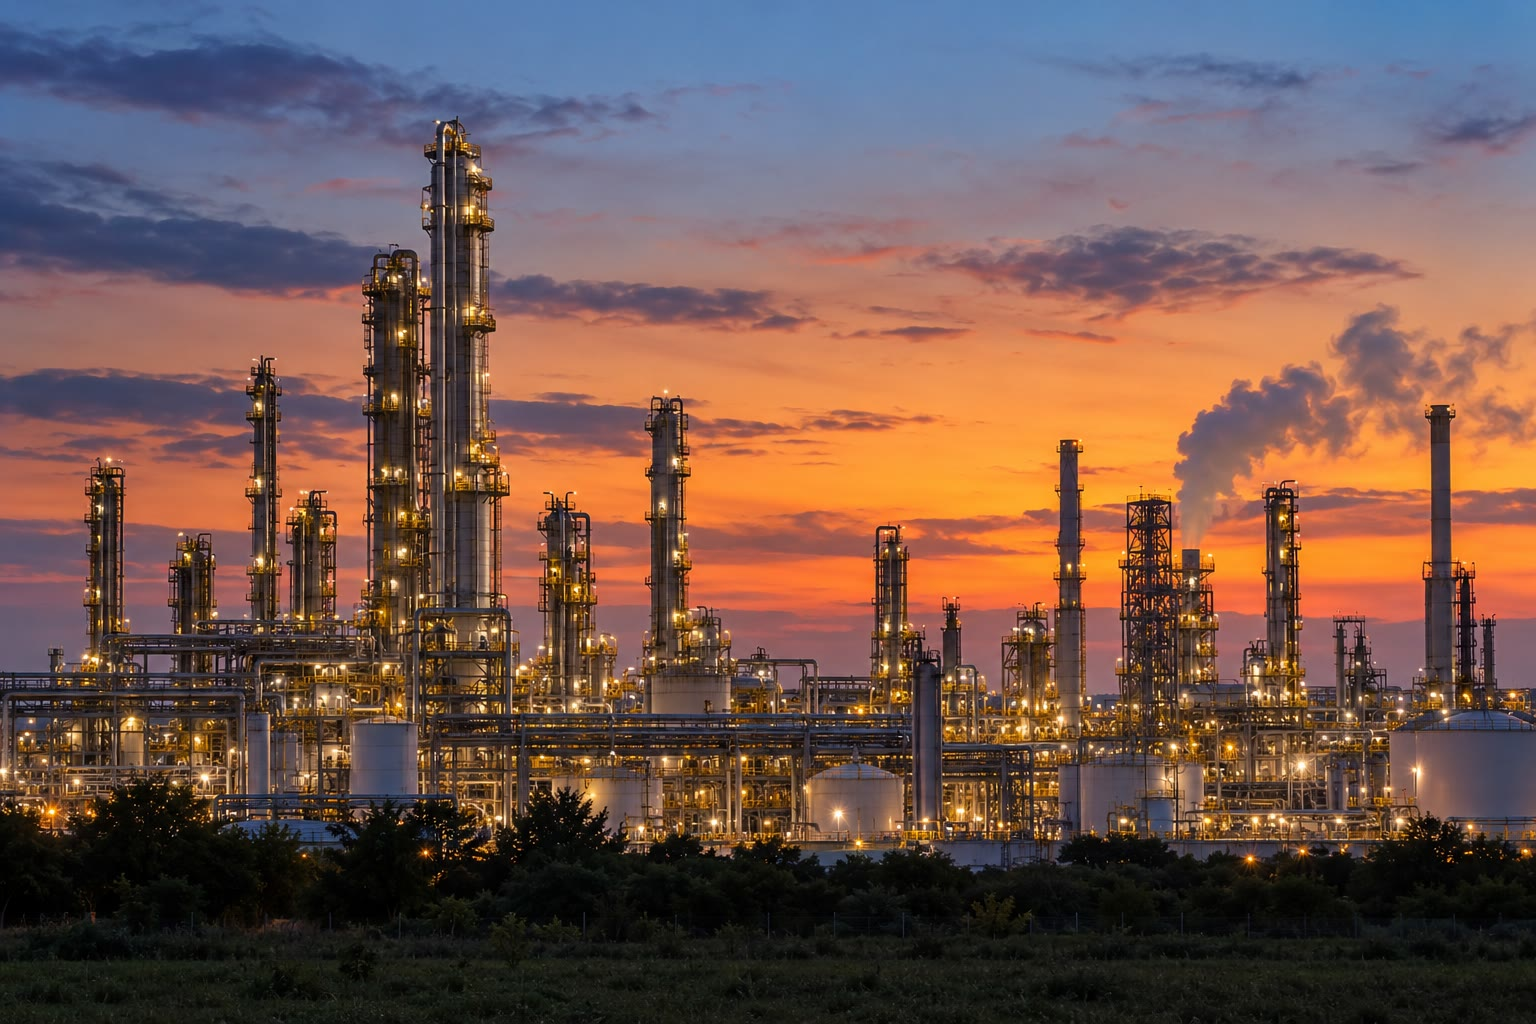
\includegraphics[width=0.6\linewidth]{images/book4/ai/b3-21-chemical-plant.jpg}

{\small Una gran planta química al anochecer. En una unidad de \omterm{def:b3:homogeneous-catalysis:carbonylation}{carbonilación}, el catalizador
es un complejo metálico disuelto en el líquido de reacción; la mayor parte de la planta
separa y recicla.}
\end{omfigure}

\section{Hidrogenación}

\begin{method}[Leer un ciclo catalítico]\label{met:b3:homogeneous-catalysis:read-cycle}
\begin{enumerate}
  \item En cada especie, contar los electrones de valencia y dar el estado de
        oxidación y el $d^n$ del metal.
  \item Nombrar cada etapa (pérdida o adición de ligando, adición oxidante,
        inserción, eliminación) y comprobar que los recuentos cambian como exige
        (adición oxidante: $+2$ en el estado de oxidación y en el recuento de electrones).
  \item Identificar el estado de reposo (la especie que se acumula) y la
        etapa determinante de la velocidad; la ley de velocidad se deduce de los preequilibrios
        entre ellos.
\end{enumerate}
\end{method}

\begin{omfigure}
\begin{tikzpicture}[font=\small, >=Stealth]
  \node (a) at (90:2.3) {\ce{RhCl(PPh3)2} \ (14, Rh$^{\mathrm I}$)};
  \node (b) at (0:3.0) {\ce{RhClH2(PPh3)2} \ (16, Rh$^{\mathrm{III}}$)};
  \node (c) at (-90:2.3) {\ce{RhClH2(RCH=CH2)(PPh3)2} \ (18)};
  \node (d) at (180:3.1) {\ce{RhClH(CH2CH2R)(PPh3)2} \ (16)};
  \draw[->, thick] (a) to[bend left=22] node[midway, above right, font=\scriptsize] {$+\,\ce{H2}$, adición oxidante} (b);
  \draw[->, thick] (b) to[bend left=22] node[midway, below right, font=\scriptsize] {$+$ alqueno} (c);
  \draw[->, thick] (c) to[bend left=22] node[midway, below left, font=\scriptsize] {inserción migratoria} (d);
  \draw[->, thick] (d) to[bend left=22] node[midway, above left, font=\scriptsize, align=right] {eliminación\\ reductora: $-$ alcano} (a);
  \node[anchor=south] (p) at (90:3.4) {\ce{RhCl(PPh3)3} \ (16, precatalizador)};
  \draw[<->, black!50] (p) -- (a) node[midway, right, font=\scriptsize] {$\mp\,\ce{PPh3}$};
\end{tikzpicture}

{\small Ciclo simplificado de la hidrogenación de alquenos con el catalizador de Wilkinson
(recuentos de electrones de valencia entre paréntesis). La pérdida de una fosfina abre una posición; el
ciclo adiciona hidrógeno, une el alqueno, lo inserta en un enlace Rh--H y
elimina el alcano.}
\end{omfigure}

\begin{proposition}[Cinética de Wilkinson]\label{prop:b3:homogeneous-catalysis:wilkinson-rate}
Si $\ce{RhClL3} \rightleftharpoons \ce{RhClL2} + \mathrm L$ ($K_1$) y $\ce{RhClL2} + \ce{H2} \rightleftharpoons \ce{RhClH2L2}$ ($K_2$) son equilibrios
rápidos y la reacción del dihidruro con el alqueno (constante de velocidad $k$)
es determinante de la velocidad,
\[
  v = \frac{kK_1K_2[\mathrm{Rh}]_{\mathrm{tot}}[\ce{H2}][\text{alqueno}]}{[\mathrm L] + K_1 + K_1K_2[\ce{H2}]},
\]
que se satura en hidrógeno y se inhibe al añadir fosfina L.
\end{proposition}

\begin{proof}
$[\ce{RhClL2}] = K_1[\ce{RhClL3}]/[\mathrm L]$ y $[\ce{RhClH2L2}] = K_2[\ce{H2}][\ce{RhClL2}]$. Escribiendo $[\mathrm{Rh}]_{\mathrm{tot}}$ como la
suma de las tres especies y despejando la concentración del dihidruro, se obtiene $[\ce{RhClH2L2}] =
K_1K_2[\ce{H2}][\mathrm{Rh}]_{\mathrm{tot}}/([\mathrm L] + K_1 + K_1K_2[\ce{H2}])$; la velocidad es $k$ por esta cantidad y por la concentración
de alqueno.
\end{proof}

El catalizador de Wilkinson hidrogena los alquenos no impedidos mucho más deprisa que
los sustituidos y no toca los grupos carbonilo: la selectividad de un
centro metálico congestionado. Las difosfinas quirales convierten la misma química en
hidrogenación asimétrica (\cref{ch:b3:asymmetric-synthesis}).

\section{Procesos de carbonilación}

\begin{definition}[Hidroformilación]\label{def:b3:homogeneous-catalysis:hydroformylation}
La \emph{hidroformilación}\index{hidroformilacion@hidroformilación} es la adición de un átomo de hidrógeno
y de un grupo formilo (CHO) a un doble enlace C=C, a partir de $\ce{H2}$ y CO, que convierte un
alqueno en un aldehído con un carbono más. La \emph{razón
lineal/ramificado}\index{razon lineal/ramificado@razón lineal/ramificado} es la razón entre el aldehído de cadena
lineal y el ramificado.
\end{definition}

Los primeros procesos usaban $\ce{HCo(CO)4}$ a unos 150 a \qty{180}{\celsius} y presiones muy
altas. El rodio con trifenilfosfina trabaja a unos \qty{100}{\celsius} y a
presiones mucho más bajas, y da una \omterm{def:b3:homogeneous-catalysis:hydroformylation}{razón lineal/ramificado} mayor: las fosfinas
voluminosas favorecen la inserción que sitúa el metal sobre el carbono terminal.
El propeno da butanal, que se hidrogena a butanol o se convierte en alcoholes
plastificantes.

\begin{definition}[Carbonilación]\label{def:b3:homogeneous-catalysis:carbonylation}
La \emph{carbonilación}\index{carbonilacion@carbonilación} es la introducción de un grupo carbonilo
en una molécula por reacción con monóxido de carbono, catalizada por un complejo metálico
mediante la inserción migratoria del CO.
\end{definition}

La \omterm{def:b3:homogeneous-catalysis:carbonylation}{carbonilación} del metanol a ácido acético, $\ce{CH3OH + CO -> CH3COOH}$, funciona con
rodio (el proceso Monsanto) o con iridio (el proceso Cativa), con yoduro de metilo
como cocatalizador: el yoduro de hidrógeno convierte el metanol en yoduro de metilo, el metal
inserta CO en el grupo metilo, y el yoduro de acetilo formado se hidroliza y
libera de nuevo HI.

\begin{omfigure}
\begin{tikzpicture}[font=\small, >=Stealth]
  \node (a) at (90:2.1) {$\ce{[M(CO)2I2]-}$ (16)};
  \node (b) at (0:2.9) {$\ce{[CH3M(CO)2I3]-}$ (18)};
  \node (c) at (-90:2.1) {$\ce{[CH3COM(CO)I3]-}$ (16)};
  \node (d) at (180:2.9) {$\ce{[CH3COM(CO)2I3]-}$ (18)};
  \draw[->, thick] (a) to[bend left=22] node[midway, above right, font=\scriptsize, align=left] {$+\,\ce{CH3I}$\\ adición oxidante} (b);
  \draw[->, thick] (b) to[bend left=22] node[midway, below right, font=\scriptsize] {inserción migratoria} (c);
  \draw[->, thick] (c) to[bend left=22] node[midway, below left, font=\scriptsize] {$+$ CO} (d);
  \draw[->, thick] (d) to[bend left=22] node[midway, above left, font=\scriptsize, align=right] {eliminación reductora\\ $-\,\ce{CH3COI}$} (a);
  \node[anchor=north, align=center, font=\scriptsize] at (0,-2.55) {$\ce{CH3COI + H2O -> CH3COOH + HI}$, \quad $\ce{CH3OH + HI -> CH3I + H2O}$};
\end{tikzpicture}

{\small El ciclo de \omterm{def:b3:homogeneous-catalysis:carbonylation}{carbonilación} del metanol para $\mathrm M = \mathrm{Rh}$ (Monsanto); recuentos de electrones de
valencia entre paréntesis, estado de oxidación del metal I arriba y III en los demás casos.
Con el rodio, la adición oxidante del yoduro de metilo es determinante de la velocidad. Con el
iridio (Cativa) es mucho más rápida, la inserción migratoria es lenta, y unos
\omterm{def:b3:surfaces-catalysis:catalyst-design}{promotores} que retiran un yoduro del $\ce{[CH3Ir(CO)2I3]-}$ aceleran la inserción.}
\end{omfigure}

\begin{proposition}[Ley de velocidad del proceso del rodio]\label{prop:b3:homogeneous-catalysis:monsanto-rate}
Si la adición oxidante del yoduro de metilo al $\ce{[Rh(CO)2I2]-}$ es determinante de la velocidad y
este complejo es el estado de reposo, $v = k[\mathrm{Rh}]_{\mathrm{tot}}[\ce{CH3I}]$: de orden cero respecto del CO y del
metanol.
\end{proposition}

\begin{proof}
La velocidad es la de la etapa lenta, $k[\ce{[Rh(CO)2I2]-}][\ce{CH3I}]$, y casi todo el rodio
está en el estado de reposo. El CO solo entra después de la etapa lenta, y el metanol solo
regenera el yoduro de metilo, cuya concentración estacionaria la fija el yoduro
cargado en el reactor y no el metanol.
\end{proof}

El iridio se impuso al rodio en las plantas nuevas por razones prácticas: sus complejos permanecen
en disolución a concentraciones de agua más bajas, lo que ahorra energía en el secado del
producto, y dan menos subproductos. La principal reacción secundaria de ambos es la
reacción de desplazamiento del gas de agua, $\ce{CO + H2O -> CO2 + H2}$, catalizada por el mismo metal, que desperdicia
monóxido de carbono.

\section{Metátesis de olefinas}

\begin{definition}[Metátesis de olefinas]\label{def:b3:homogeneous-catalysis:metathesis}
La \emph{metátesis de olefinas}\index{metatesis de olefinas@metátesis de olefinas} es el intercambio de las
mitades alquilideno de dos alquenos, $\mathrm{RCH{=}CHR + R'CH{=}CHR' \rightleftharpoons 2\,RCH{=}CHR'}$, catalizado por
\omterm{def:b3:organometallic-bonding:carbene}{complejos carbénicos} metálicos a través de un \emph{metalaciclobutano}\index{metalaciclobutano},
un anillo de cuatro miembros formado por el metal y tres carbonos. Sus formas sintéticas son la
\emph{metátesis por cierre de anillo}\index{metatesis por cierre de anillo@metátesis por cierre de anillo} (RCM), que une
dos extremos alquénicos de una molécula en un anillo con pérdida de eteno, la
\emph{polimerización por metátesis con apertura de anillo}\index{polimerizacion por metatesis con apertura de anillo@polimerización por metátesis con apertura de anillo}
(ROMP) de alquenos cíclicos tensionados, y la \emph{metátesis
cruzada}\index{metatesis cruzada@metátesis cruzada} entre dos alquenos distintos.
\end{definition}

\begin{definition}[Mecanismo de Chauvin]\label{def:b3:homogeneous-catalysis:chauvin}
El \emph{mecanismo de Chauvin}\index{mecanismo de Chauvin} de la metátesis es la
cicloadición $[2+2]$ de un alqueno a un \omterm{def:b3:organometallic-bonding:carbene}{carbeno} metálico, $\mathrm{[M]{=}CHR}$, que da un
\omterm{def:b3:homogeneous-catalysis:metathesis}{metalaciclobutano}, seguida de su cicloreversión en el otro sentido,
que libera un alqueno nuevo y un \omterm{def:b3:organometallic-bonding:carbene}{carbeno} nuevo.
\end{definition}

\begin{omfigure}
\setchemfig{atom sep=2.1em}
\schemestart
\chemfig{M=[:0]CHR}
\+
\chemfig{R'HC=[:0]CHR'}
\arrow{<=>}
\chemfig{M?-[:0]CHR-[:-90]CHR'-[:180]CHR'?}
\arrow{<=>}
\chemfig{M=[:0]CHR'}
\+
\chemfig{RHC=[:0]CHR'}
\schemestop
\par\vspace{10pt}

{\small El \omterm{def:b3:homogeneous-catalysis:chauvin}{mecanismo de Chauvin}: un \omterm{def:b3:organometallic-bonding:carbene}{carbeno} metálico y un alqueno se combinan en un
\omterm{def:b3:homogeneous-catalysis:metathesis}{metalaciclobutano}, que se abre en el otro sentido para dar un \omterm{def:b3:organometallic-bonding:carbene}{carbeno} nuevo y un alqueno
nuevo. Cada etapa es reversible: la metátesis alcanza un equilibrio salvo que un
producto se vaya.}
\end{omfigure}

\begin{proposition}[Desplazar la metátesis por cierre de anillo]\label{prop:b3:homogeneous-catalysis:metathesis-equilibrium}
Para un cierre de anillo $\text{dieno} \rightleftharpoons \text{cicloalqueno} + \ce{C2H4}$, eliminar el eteno de la
disolución lleva la reacción hasta el final; la reacción está favorecida por la
entropía de liberar una molécula de gas.
\end{proposition}

\begin{proof}
En el equilibrio, $K = [\text{anillo}][\ce{C2H4}]/[\text{dieno}]$: si $[\ce{C2H4}]$ se mantiene baja purgando o
haciendo el vacío, $[\text{anillo}]/[\text{dieno}] = K/[\ce{C2H4}]$ crece sin límite. El número de moléculas
aumenta en uno en la reacción, mientras que los enlaces formados y rotos (un C=C cada uno) son
análogos: $\Delta_rH^\circ \approx 0$ para un anillo sin tensión y $\Delta_rS^\circ > 0$, de modo que $K$ es favorable.
\end{proof}

La ROMP de anillos tensionados, como el norborneno, va en el otro sentido por la razón
opuesta: la liberación de la tensión de anillo paga la pérdida de entropía de traslación.
Los \omterm{def:b3:organometallic-bonding:carbene}{carbenos} de rutenio de Robert Grubbs toleran el agua, el aire y la mayoría de los grupos
funcionales; los alquilidenos de molibdeno y de wolframio de Richard Schrock son más activos
y pueden hacerse enantioselectivos.

\section{Acoplamiento cruzado con paladio}

\begin{definition}[Reacciones de acoplamiento cruzado]\label{def:b3:homogeneous-catalysis:cross-coupling}
Una \emph{reacción de acoplamiento cruzado}\index{reaccion de acoplamiento cruzado@reacción de acoplamiento cruzado} une dos
fragmentos carbonados distintos, un haluro orgánico y un reactivo organometálico o un
alqueno, sobre un catalizador metálico, normalmente de paladio. En la \emph{reacción de
Heck}\index{reaccion de Heck@reacción de Heck}, un haluro de arilo o de vinilo se acopla con un alqueno,
lo que da un alqueno sustituido; en el \emph{acoplamiento de
Suzuki--Miyaura}\index{acoplamiento de Suzuki--Miyaura}, se acopla con un compuesto
organoborado en presencia de una base.
\end{definition}

\begin{omfigure}
\begin{tikzpicture}[font=\small, >=Stealth]
  \node (a) at (90:2.0) {$\mathrm{Pd^0L_2}$};
  \node (b) at (0:2.6) {$\mathrm{ArPd^{II}XL_2}$};
  \node (c) at (-90:2.0) {$\mathrm{ArPd^{II}Ar'L_2}$};
  \draw[->, thick] (a) to[bend left=25] node[midway, above right, font=\scriptsize, align=left] {$+\,$ArX\\ adición oxidante} (b);
  \draw[->, thick] (b) to[bend left=25] node[midway, below right, font=\scriptsize, align=left] {$+\,\mathrm{Ar'B(OH)_2}$, base\\ transmetalación} (c);
  \draw[->, thick] (c) to[bend left=35] node[midway, left, font=\scriptsize, align=right] {eliminación reductora\\ $-\,$Ar--Ar$'$} (a);
\end{tikzpicture}

{\small El ciclo de Suzuki--Miyaura: el paladio(0) se inserta en el enlace C--X del
haluro de arilo, recibe el segundo grupo arilo del ácido borónico activado por
la base y libera el biarilo por eliminación reductora.}
\end{omfigure}

\begin{method}[Elegir un acoplamiento cruzado]\label{met:b3:homogeneous-catalysis:choose-coupling}
\begin{enumerate}
  \item Desconectar la molécula objetivo por el enlace C--C que se va a formar; uno de los compañeros pasa a ser el
        haluro (yoduro $>$ bromuro $>$ triflato $>$ cloruro en reactividad), y el otro, el
        ácido borónico (Suzuki--Miyaura), el alqueno (Heck), el organocíncico
        (Negishi) o el alquino terminal con cobre(I) (Sonogashira).
  \item Preferir el par de compañeros cuyos reactivos sean estables, disponibles y lo menos
        tóxicos posible: ácidos borónicos para los biarilos.
  \item Elegir el ligando para la etapa más difícil: las fosfinas voluminosas y ricas en electrones
        o los \omterm{def:b3:organometallic-bonding:carbene}{carbenos N-heterocíclicos} aceleran la adición oxidante de los cloruros.
  \item Planificar la eliminación del paladio del producto hasta los niveles bajos
        permitidos en los fármacos (resinas captadoras, cristalización).
\end{enumerate}
\end{method}

\section{Catálisis de polimerización}

\begin{definition}[Catálisis de Ziegler--Natta]\label{def:b3:homogeneous-catalysis:ziegler-natta}
Un \emph{catalizador de Ziegler--Natta}\index{catalizador de Ziegler--Natta} polimeriza
alquenos a baja presión; se prepara a partir de un haluro de un metal de transición, normalmente de
titanio, y de un compuesto de alquilaluminio. El \emph{mecanismo de
Cossee--Arlman}\index{mecanismo de Cossee--Arlman} del crecimiento de la cadena es la coordinación
del alqueno en una posición vacante en cis respecto de la cadena alquílica en crecimiento sobre el metal,
seguida de su inserción migratoria en el enlace metal--carbono, que deja de nuevo una
posición vacante. Un \emph{catalizador de sitio único}\index{catalizador de sitio unico@catalizador de sitio único} tiene
todos sus centros activos idénticos, como en un catalizador metalocénico molecular.
\end{definition}

\begin{omfigure}
\begin{tikzpicture}[font=\small, >=Stealth]
  \begin{scope}[every node/.style={inner sep=1pt}]
  % panel 1: chain and vacant site
  \node (m1) at (0,0) {M};
  \node (p1) at (-0.7,0.55) {P};
  \node (v1) at (0.7,0.55) {$\square$};
  \draw (m1) -- (p1);
  % panel 2: alkene bound side-on at the vacant site
  \node (m2) at (3.6,0) {M};
  \node (p2) at (2.9,0.55) {P};
  \node (c2a) at (4.75,1.25) {\ce{CH2}};
  \node (c2b) at (4.75,0.25) {\ce{CH2}};
  \draw (m2) -- (p2);
  \draw[double, double distance=1.6pt] (c2a) -- (c2b);
  \draw[dashed] (m2) -- (4.55,0.75);
  % panel 3: chain longer by two carbons, vacant site moved
  \node (m3) at (7.7,0) {M};
  \node (v3) at (7.0,0.55) {$\square$};
  \node (c3a) at (8.45,0.55) {\ce{CH2}};
  \node (c3b) at (8.45,1.45) {\ce{CH2}};
  \node (p3) at (7.75,1.95) {P};
  \draw (m3) -- (c3a) -- (c3b) -- (p3);
  \end{scope}
  \draw[->, thick] (1.25,0.35) -- (2.55,0.35) node[midway, above, font=\scriptsize] {$+\,\ce{C2H4}$};
  \draw[->, thick] (5.35,0.35) -- (6.3,0.35) node[midway, above, font=\scriptsize] {inserción};
\end{tikzpicture}
\par\medskip

{\small El \omterm{def:b3:homogeneous-catalysis:ziegler-natta}{mecanismo de Cossee--Arlman} (P: la cadena polimérica en crecimiento; $\square$: una
posición vacante). El alqueno se une junto a la cadena y se inserta en el enlace M--C
a través de un estado de transición de cuatro centros; la cadena, dos carbonos
más larga, ocupa ahora la posición en la que estaba el alqueno, y la posición vacante se ha
desplazado.}
\end{omfigure}

\begin{proposition}[La tacticidad a partir de la simetría del catalizador]\label{prop:b3:homogeneous-catalysis:tacticity-symmetry}
Para un catalizador metalocénico en el que la cadena migra entre dos posiciones de coordinación
en cada inserción, un catalizador de simetría $C_2$ da polipropileno isotáctico, y uno de simetría $C_s$,
polipropileno sindiotáctico.
\end{proposition}

\begin{proof}[Argumento]
La cara del propeno que se inserta la elige el entorno quiral de la
posición. En un catalizador de simetría $C_2$, las dos posiciones se intercambian por el eje $C_2$,
que conserva la quiralidad (\cref{ch:b3:point-groups}): ambas posiciones seleccionan la
misma cara, y los grupos metilo sucesivos tienen la misma configuración (isotáctico).
En un catalizador de simetría $C_s$, las dos posiciones son imágenes especulares: seleccionan caras
opuestas, y las configuraciones alternan (sindiotáctico). Un catalizador cuyas posiciones
son aquirales, como el $\ce{Cp2ZrCl2}$ sin puente con metilaluminoxano, da un polímero
atáctico.
\end{proof}

\begin{proposition}[Distribución de Schulz--Flory]\label{prop:b3:homogeneous-catalysis:schulz-flory}
Si cada cadena en crecimiento sobre un \omterm{def:b3:homogeneous-catalysis:ziegler-natta}{catalizador de sitio único} añade un monómero con una
probabilidad constante $p$ y, en caso contrario, se transfiere (se termina), la fracción en número de
cadenas de $n$ unidades es $x_n = (1 - p)p^{n-1}$, y la dispersidad $M_w/M_n = 1 + p$ tiende a 2 para las cadenas largas.
\end{proposition}

\begin{proof}
Una cadena de exactamente $n$ unidades ha crecido $n - 1$ veces y se ha detenido una vez:
probabilidad $p^{n-1}(1 - p)$. Entonces $\sum nx_n = 1/(1 - p)$ (media en número), y las fracciones
másicas $w_n = nx_n(1 - p)$ dan la media en masa $\sum nw_n = (1 + p)/(1 - p)$. Su
cociente es $1 + p$.
\end{proof}

\begin{omfigure}
\begin{tikzpicture}
\begin{axis}[width=0.7\linewidth, height=5.2cm, xmin=0, xmax=200, ymin=0, ymax=1.05,
  axis lines=left, xlabel={$M$ / \unit{kg.mol^{-1}}}, ylabel={fracción por unidad (escalada)},
  tick label style={font=\small}, label style={font=\small},
  legend style={font=\scriptsize, draw=none, at={(0.98,0.98)}, anchor=north east}, legend cell align=left]
\addplot[omDef, line width=1pt] table[x=M_kg, y=x] {figdata/out/bachelor-3-schulz-flory.dat};
\addplot[omThm, line width=1pt] table[x=M_kg, y expr=\thisrow{w}/0.368] {figdata/out/bachelor-3-schulz-flory.dat};
\draw[black!40, dashed] (axis cs:28.05,0) -- (axis cs:28.05,1);
\node[font=\scriptsize, anchor=west] at (axis cs:30,0.5) {$M_n$};
\legend{fracción en número, fracción másica (escalada a su máximo)}
\end{axis}
\end{tikzpicture}

{\small La distribución de masas molares más probable de un polietileno obtenido con un
\omterm{def:b3:homogeneous-catalysis:ziegler-natta}{catalizador de sitio único} (modelo: grado de polimerización medio 1000): la fracción en
número decae exponencialmente, y la fracción másica alcanza su máximo en $M_n \approx \qty{28}{kg/mol}$; $M_w = 2M_n$. Los \omterm{def:b3:homogeneous-catalysis:ziegler-natta}{catalizadores
de Ziegler--Natta} clásicos, con varios tipos de sitios, dan distribuciones
más anchas.}
\end{omfigure}

\begin{inthelab}[Un acoplamiento de Suzuki y su paladio]
El bromuro de arilo, el ácido borónico (1.2 equivalentes), el carbonato de potasio y unas
décimas de por ciento de un complejo fosfina--paladio se agitan en una
mezcla desgasificada de tolueno, etanol y agua bajo nitrógeno a reflujo. Tras
el tratamiento, el biarilo bruto se agita con una sílice funcionalizada con tioles que
fija el paladio, se filtra y se cristaliza; el paladio residual se mide por
espectrometría de masas con plasma.
\end{inthelab}

\begin{safety}{\ghs[0.62cm]{GHS02}\ghs[0.62cm]{GHS04}\ghs[0.62cm]{GHS06}\ghs[0.62cm]{GHS08}}
% ledger: ghs4:MeI, ghs:CO
Yoduro de metilo: tóxico por inhalación y por ingestión, nocivo en contacto con la piel, se sospecha que
provoca cáncer, volátil; se manipula en una vitrina. Monóxido de carbono: extremadamente
inflamable, tóxico por inhalación, puede dañar al feto, inodoro; se usa
con detectores fijos y alarmas.
\end{safety}

\begin{history}[Ziegler, Natta y la metátesis]
Karl Ziegler descubrió en 1953 que el cloruro de titanio y los compuestos de alquilaluminio
polimerizan el eteno a presión atmosférica, y Giulio Natta, en 1954, que esos
catalizadores fabrican polipropileno estereorregular; compartieron el Premio Nobel de
Química de 1963. Yves Chauvin propuso el mecanismo del \omterm{def:b3:homogeneous-catalysis:metathesis}{metalaciclobutano} de la
metátesis en 1971; junto con Robert Grubbs y Richard Schrock, que prepararon catalizadores
de metátesis bien definidos, recibió el Premio Nobel de Química de 2005.
\end{history}

\section{Ejercicios}

\begin{exercise}[$\star$]\label{exo:b3:homogeneous-catalysis:1}
Dense el recuento de electrones de valencia y el estado de oxidación del rodio en cada etapa
del ciclo de Wilkinson de la figura.
\end{exercise}

\begin{exercise}[$\star$]\label{exo:b3:homogeneous-catalysis:2}
Nómbrense los dos aldehídos formados por \omterm{def:b3:homogeneous-catalysis:hydroformylation}{hidroformilación} del propeno. ¿Cuál es el
lineal?
\end{exercise}

\begin{exercise}[$\star$]\label{exo:b3:homogeneous-catalysis:3}
El dialilmalonato de dietilo, $\ce{(CH2=CHCH2)2C(CO2Et)2}$, experimenta una \omterm{def:b3:homogeneous-catalysis:metathesis}{metátesis por cierre de anillo}.
Dense el producto y el tamaño de su anillo.
\end{exercise}

\begin{exercise}[$\star$]\label{exo:b3:homogeneous-catalysis:4}
Dese el producto de la \omterm{def:b3:homogeneous-catalysis:cross-coupling}{reacción de Heck} del yodobenceno con acrilato de metilo, y su
configuración.
\end{exercise}

\begin{exercise}[$\star\star$]\label{exo:b3:homogeneous-catalysis:5}
A partir del ciclo del proceso del rodio, dedúzcase su ley de velocidad, y explíquese
por qué la conversión del metanol no cambia la velocidad hasta que es casi completa.
\end{exercise}

\begin{exercise}[$\star\star$]\label{exo:b3:homogeneous-catalysis:6}
Propónganse dos desconexiones de Suzuki--Miyaura del 4-metilbifenilo y elíjase una.
\end{exercise}

\begin{exercise}[$\star\star$]\label{exo:b3:homogeneous-catalysis:7}
Predígase la tacticidad del polipropileno obtenido con un catalizador de bis(indenil)circonio con puente
de simetría $C_2$, con uno de simetría $C_s$ y con $\ce{Cp2ZrCl2}$ sin puente.
\end{exercise}

\begin{exercise}[$\star\star$]\label{exo:b3:homogeneous-catalysis:8}
Con \qty{0.10}{mol\%} de catalizador, una hidrogenación alcanza un 98\,\% de conversión en \qty{2.0}{h}.
Calcúlense el número de recambio y la frecuencia de recambio media.
\end{exercise}

\begin{exercise}[$\star\star$]\label{exo:b3:homogeneous-catalysis:9}
Dibújese la unidad repetitiva del polímero obtenido por metátesis con apertura de anillo del
norborneno, y explíquese por qué la reacción llega hasta el final.
\end{exercise}

\begin{exercise}[$\star\star\star$]\label{exo:b3:homogeneous-catalysis:10}
Un \omterm{def:b3:homogeneous-catalysis:ziegler-natta}{catalizador de sitio único} da cadenas con $p = 0.9995$. Calcúlense el grado de polimerización
medio en número y la dispersidad. ¿Por qué un polímero de Ziegler--Natta tiene una distribución
más ancha?
\end{exercise}

\begin{exercise}[$\star\star\star$]\label{exo:b3:homogeneous-catalysis:11}
Demuéstrese, a partir de la ley de velocidad de Wilkinson, que la velocidad es de primer orden respecto del $\ce{H2}$ a baja presión
e independiente de él a alta presión, y que añadir fosfina ralentiza la
reacción.
\end{exercise}

\begin{exercise}[$\star\star\star$]\label{exo:b3:homogeneous-catalysis:12}
Explíquese por qué las fosfinas voluminosas elevan la \omterm{def:b3:homogeneous-catalysis:hydroformylation}{razón lineal/ramificado} en la
\omterm{def:b3:homogeneous-catalysis:hydroformylation}{hidroformilación} con rodio, y por qué una razón alta importa para los alcoholes plastificantes obtenidos
a partir de los aldehídos.
\end{exercise}

\section{Problema: del metanol al vinagre}

\begin{problem}[{Problema de fin de semana --- del metanol al vinagre en un ciclo de iridio:
los recuentos y las etapas del ciclo, su etapa determinante de la velocidad y sus promotores, la
frecuencia de recambio de una planta y el monóxido de carbono perdido en la reacción de desplazamiento del
gas de agua}]
\label{pb:b3:homogeneous-catalysis:1}
% ledger: aw:Ir, aw:C, aw:H, aw:O
Una planta de ácido acético (datos del problema) produce $\qty{5.0e5}{t}$ de ácido acético al año
en \qty{8000}{h} de funcionamiento, con \qty{200}{m^3} de líquido de reacción que contiene \qty{5.0}{mmol/L} de
iridio. Su selectividad respecto del monóxido de carbono es del 94\,\%: el resto se convierte por la
reacción de desplazamiento del gas de agua.

\medskip\noindent\textbf{Parte I --- El ciclo.}
\begin{enumerate}
  \item Cuéntense los electrones del $\ce{[Ir(CO)2I2]-}$ y dese su estado de oxidación.
  \item Adición oxidante del $\ce{CH3I}$: ¿producto, recuento, estado de oxidación?
  \item Pérdida de yoduro y adición de CO: ¿qué complejo neutro se forma?
  \item Inserción migratoria: ¿producto y recuento?
  \item Adición de yoduro y después eliminación reductora de yoduro de acetilo: ¿qué se
        regenera?
  \item Escríbanse las dos etapas orgánicas que cierran el ciclo con agua y metanol.
  \item Escríbase la reacción global.
\end{enumerate}

\medskip\noindent\textbf{Parte II --- Cinética.}
\begin{enumerate}[resume]
  \item ¿Qué etapa es determinante de la velocidad con el iridio, y en qué difiere del
        rodio?
  \item ¿Cómo aceleran el ciclo los \omterm{def:b3:surfaces-catalysis:catalyst-design}{promotores} que capturan yoduro?
  \item ¿Qué dependencia de la concentración de yoduro predice esto?
  \item ¿Por qué la velocidad es independiente de la concentración de metanol?
\end{enumerate}

\medskip\noindent\textbf{Parte III --- La planta.}
\begin{enumerate}[resume]
  \item Calcúlese la cantidad de ácido acético producida al año.
  \item Calcúlese la cantidad por hora.
  \item Calcúlese la cantidad de iridio en el reactor, y su masa.
  \item Calcúlese la frecuencia de recambio.
  \item Calcúlese el número de recambio por año.
  \item Calcúlese el rendimiento espacio--tiempo en kilogramos por metro cúbico y por hora.
\end{enumerate}

\medskip\noindent\textbf{Parte IV --- La reacción de desplazamiento del gas de agua.}
\begin{enumerate}[resume]
  \item Escríbase la reacción de desplazamiento del gas de agua.
  \item Calcúlese el CO consumido por mol de ácido acético.
  \item Calcúlese el \ce{CO2} formado por mol de ácido acético.
  \item Calcúlese la masa de \ce{CO2} emitida por tonelada de ácido acético.
  \item ¿Por qué ayuda trabajar a una concentración de agua más baja, y qué lo limita?
  \item ¿Qué otro producto da la reacción de desplazamiento, y por qué es un problema en el
        reactor?
  \item Enúnciese el resultado: la frecuencia de recambio del catalizador de iridio.
\end{enumerate}
\end{problem}
